\documentclass[10pt]{beamer}
\usepackage[utf8]{inputenc}
\usepackage{listings}
\usepackage{xcolor}

\usepackage{amsmath}
\usepackage{nccmath}
%\usepackage{showframe}
\usepackage{amssymb} 
\usetheme[progressbar=frametitle]{metropolis}
\usepackage{appendixnumberbeamer}
\usepackage{booktabs}
\usepackage[scale=2]{ccicons}

\usepackage{pgfplots}
\usepgfplotslibrary{dateplot}

\usepackage{xspace}
\newcommand{\themename}{\textbf{\textsc{metropolis}}\xspace}

\title{6 Algorithmic Journeys with Concepts}
%\subtitle{Generic algorithms and performance}
% \date{\today}
\date{}
\author{Taras Shevchenko}
\institute{Rails Reactor / Giphy}
% \titlegraphic{\hfill\includegraphics[height=1.5cm]{logo.pdf}}
\lstdefinestyle{cpp}{
  language=C++,
  stepnumber=1,
  numbersep=10pt,
  tabsize=2,
  showspaces=false,
  showstringspaces=false,
  basicstyle=\scriptsize,
  breaklines
}

\begin{document}

\maketitle

%\begin{frame}{Table of contents}
%  \setbeamertemplate{section in toc}[sections numbered]
%  \tableofcontents[hideallsubsections]
%\end{frame}


\begin{frame}{The Software Industry is Not Industrialized}
    \begin{columns}
        \begin{column}{0.6\textwidth}
			Software components (routines), to be widely applicable to
			different machines and users, should be available in families arranged
			according to precision, robustness, generality and time-space performance.
        \end{column}
        \begin{column}{0.4\textwidth}  %%<--- here
                \begin{center}
					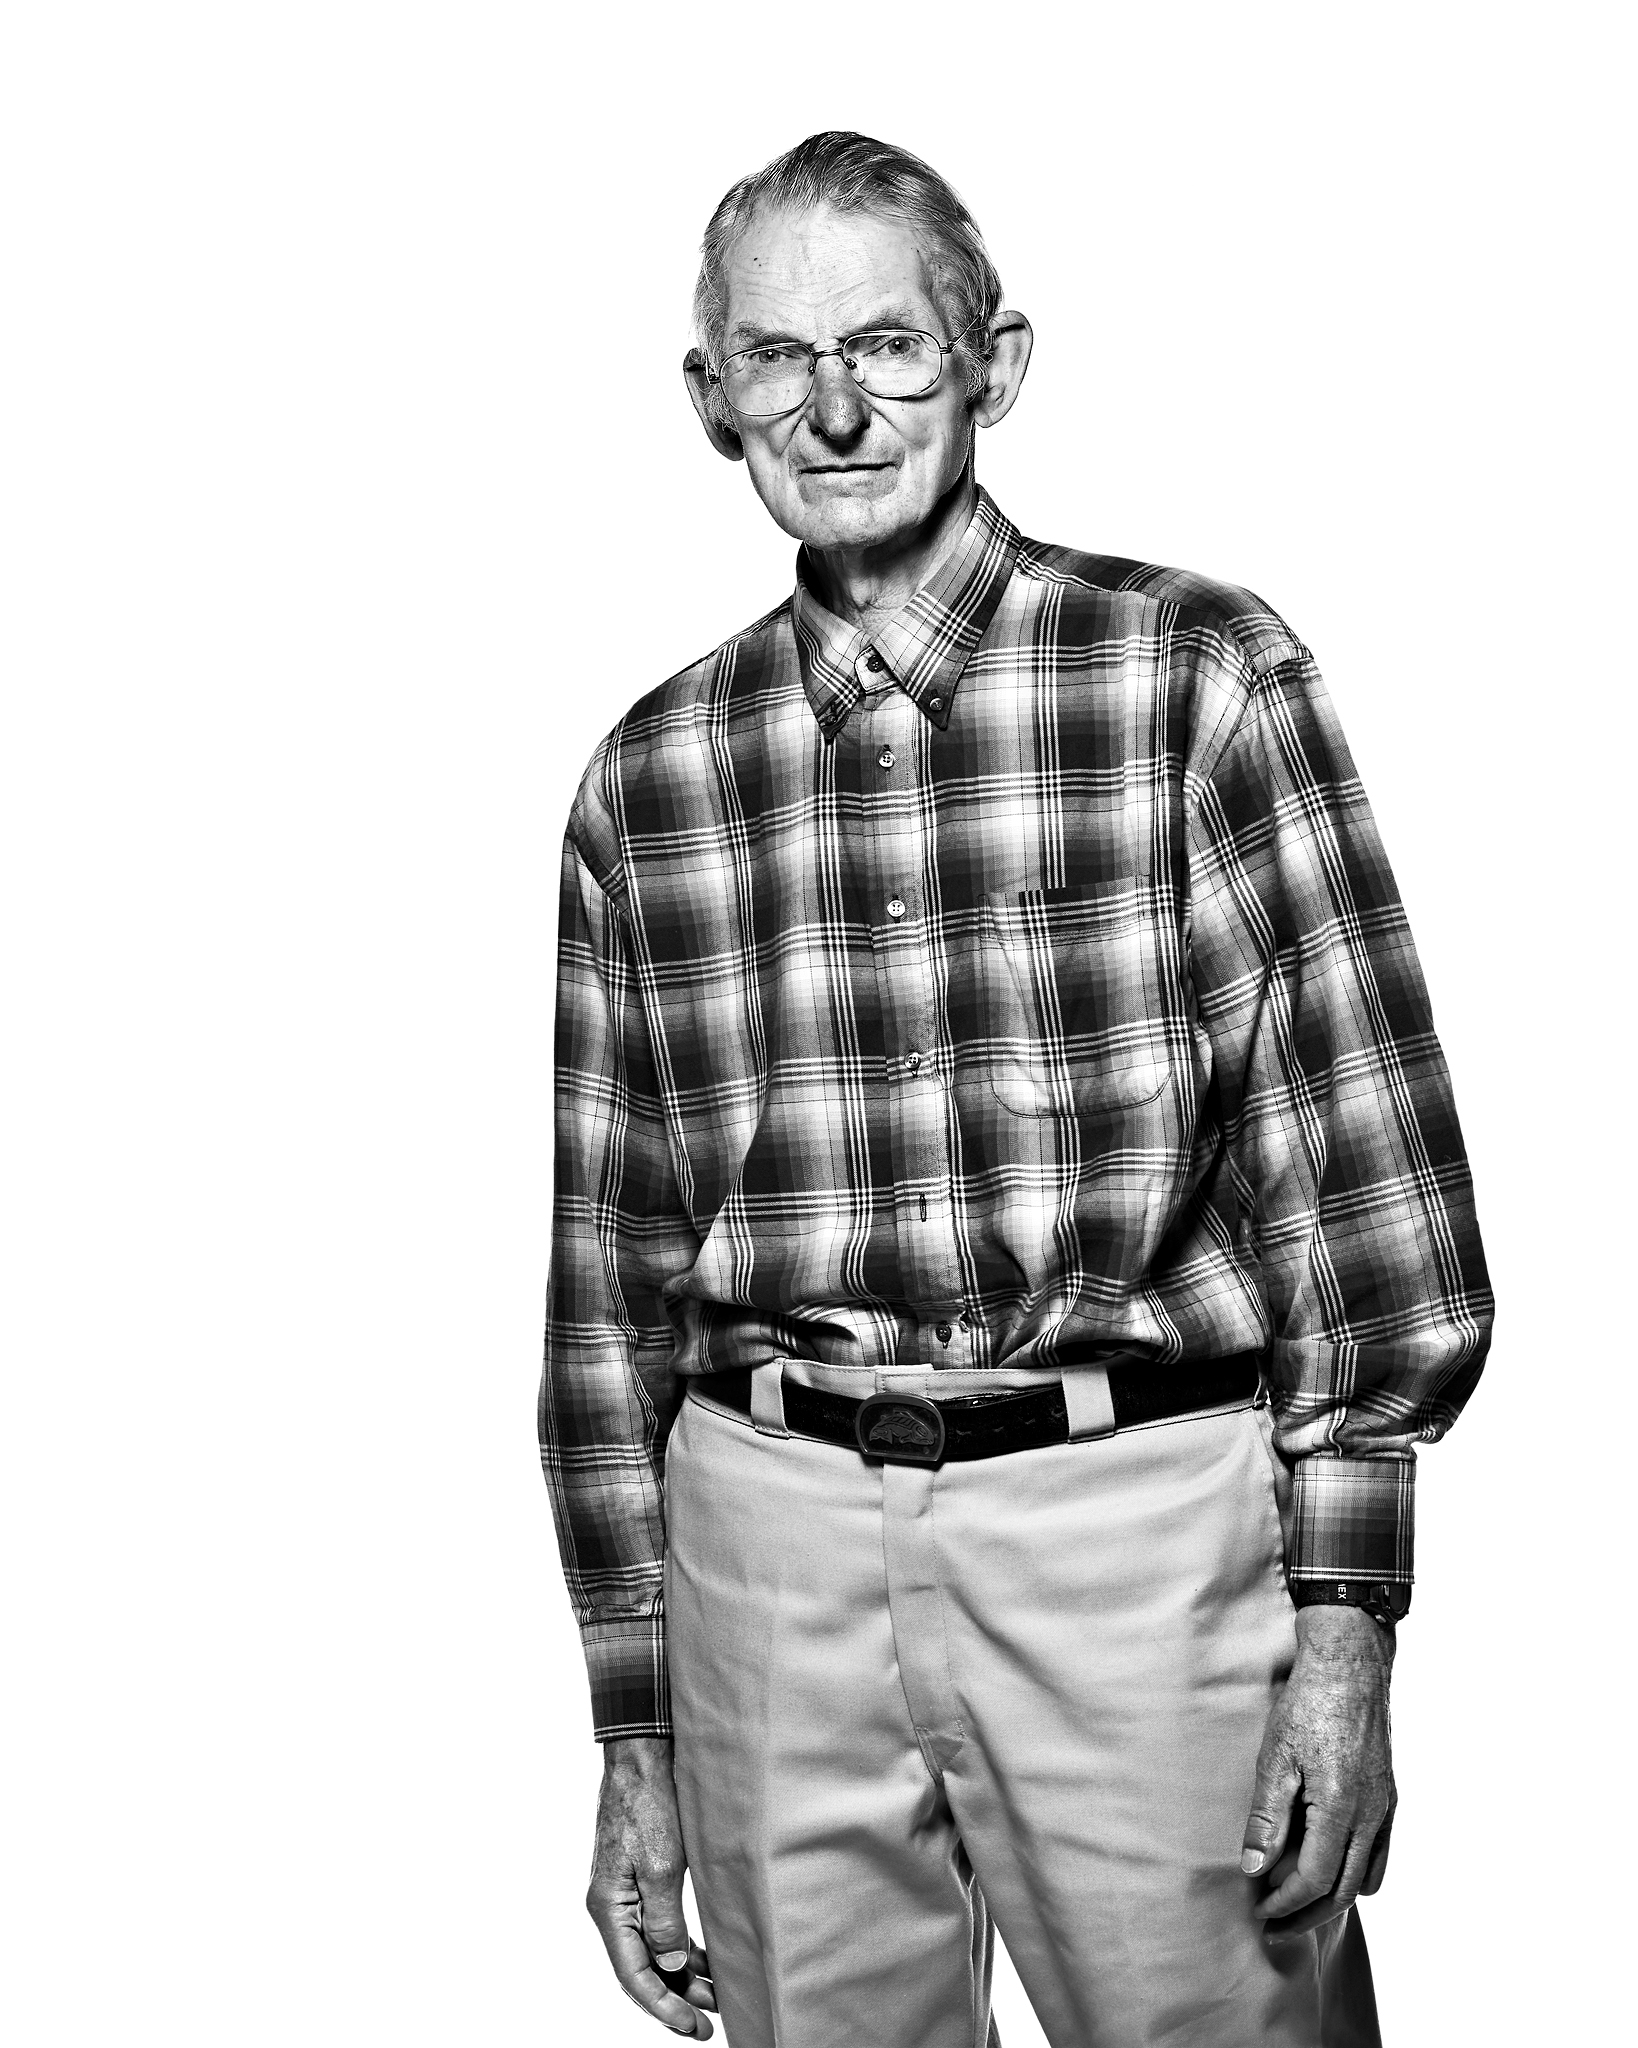
\includegraphics[height=5cm]{images/doug_mcilroy.jpg}
                \end{center}
        \end{column}
    \end{columns}
\end{frame}

\begin{frame}{A Familiar Example. Douglas McIlroy about sin}
Dimensions along which we wish to have variablity:
\begin{enumerate}
    \item precision, for which perhaps ten different approximating functionsmight suffice
    \item floating vs fixed computation
    \item argument ranges $[0, \pi/2]$, $[0, 2pi]$, also $[-\pi/2, pi/2]$, $[-\pi, \pi]$, $[-big, +big]$
    \item robustness - ranging from no argument validation through signaling of complete loss of significance, to signaling of specified range violations
\end{enumerate}

\end{frame}

\begin{frame}{Douglas McIlroy}
    \begin{columns}
        \begin{column}{0.6\textwidth}
            \begin{enumerate}
                \item Choices
                    \begin{enumerate}
                        \item precision
                        \item robustness
                        \item generality
                        \item generality
                        \item algorithm
                        \item interfaces and error-handling
                    \end{enumerate}
                \item Application Areas
                \begin{enumerate}
                    \item numerical approximation
                    \item I/O
                    \item 2d and 3d geometry
                    \item text processing
                    \item storage management
                \end{enumerate}
            \end{enumerate}

        \end{column}
        \begin{column}{0.4\textwidth}  %%<--- here
                \begin{center}
					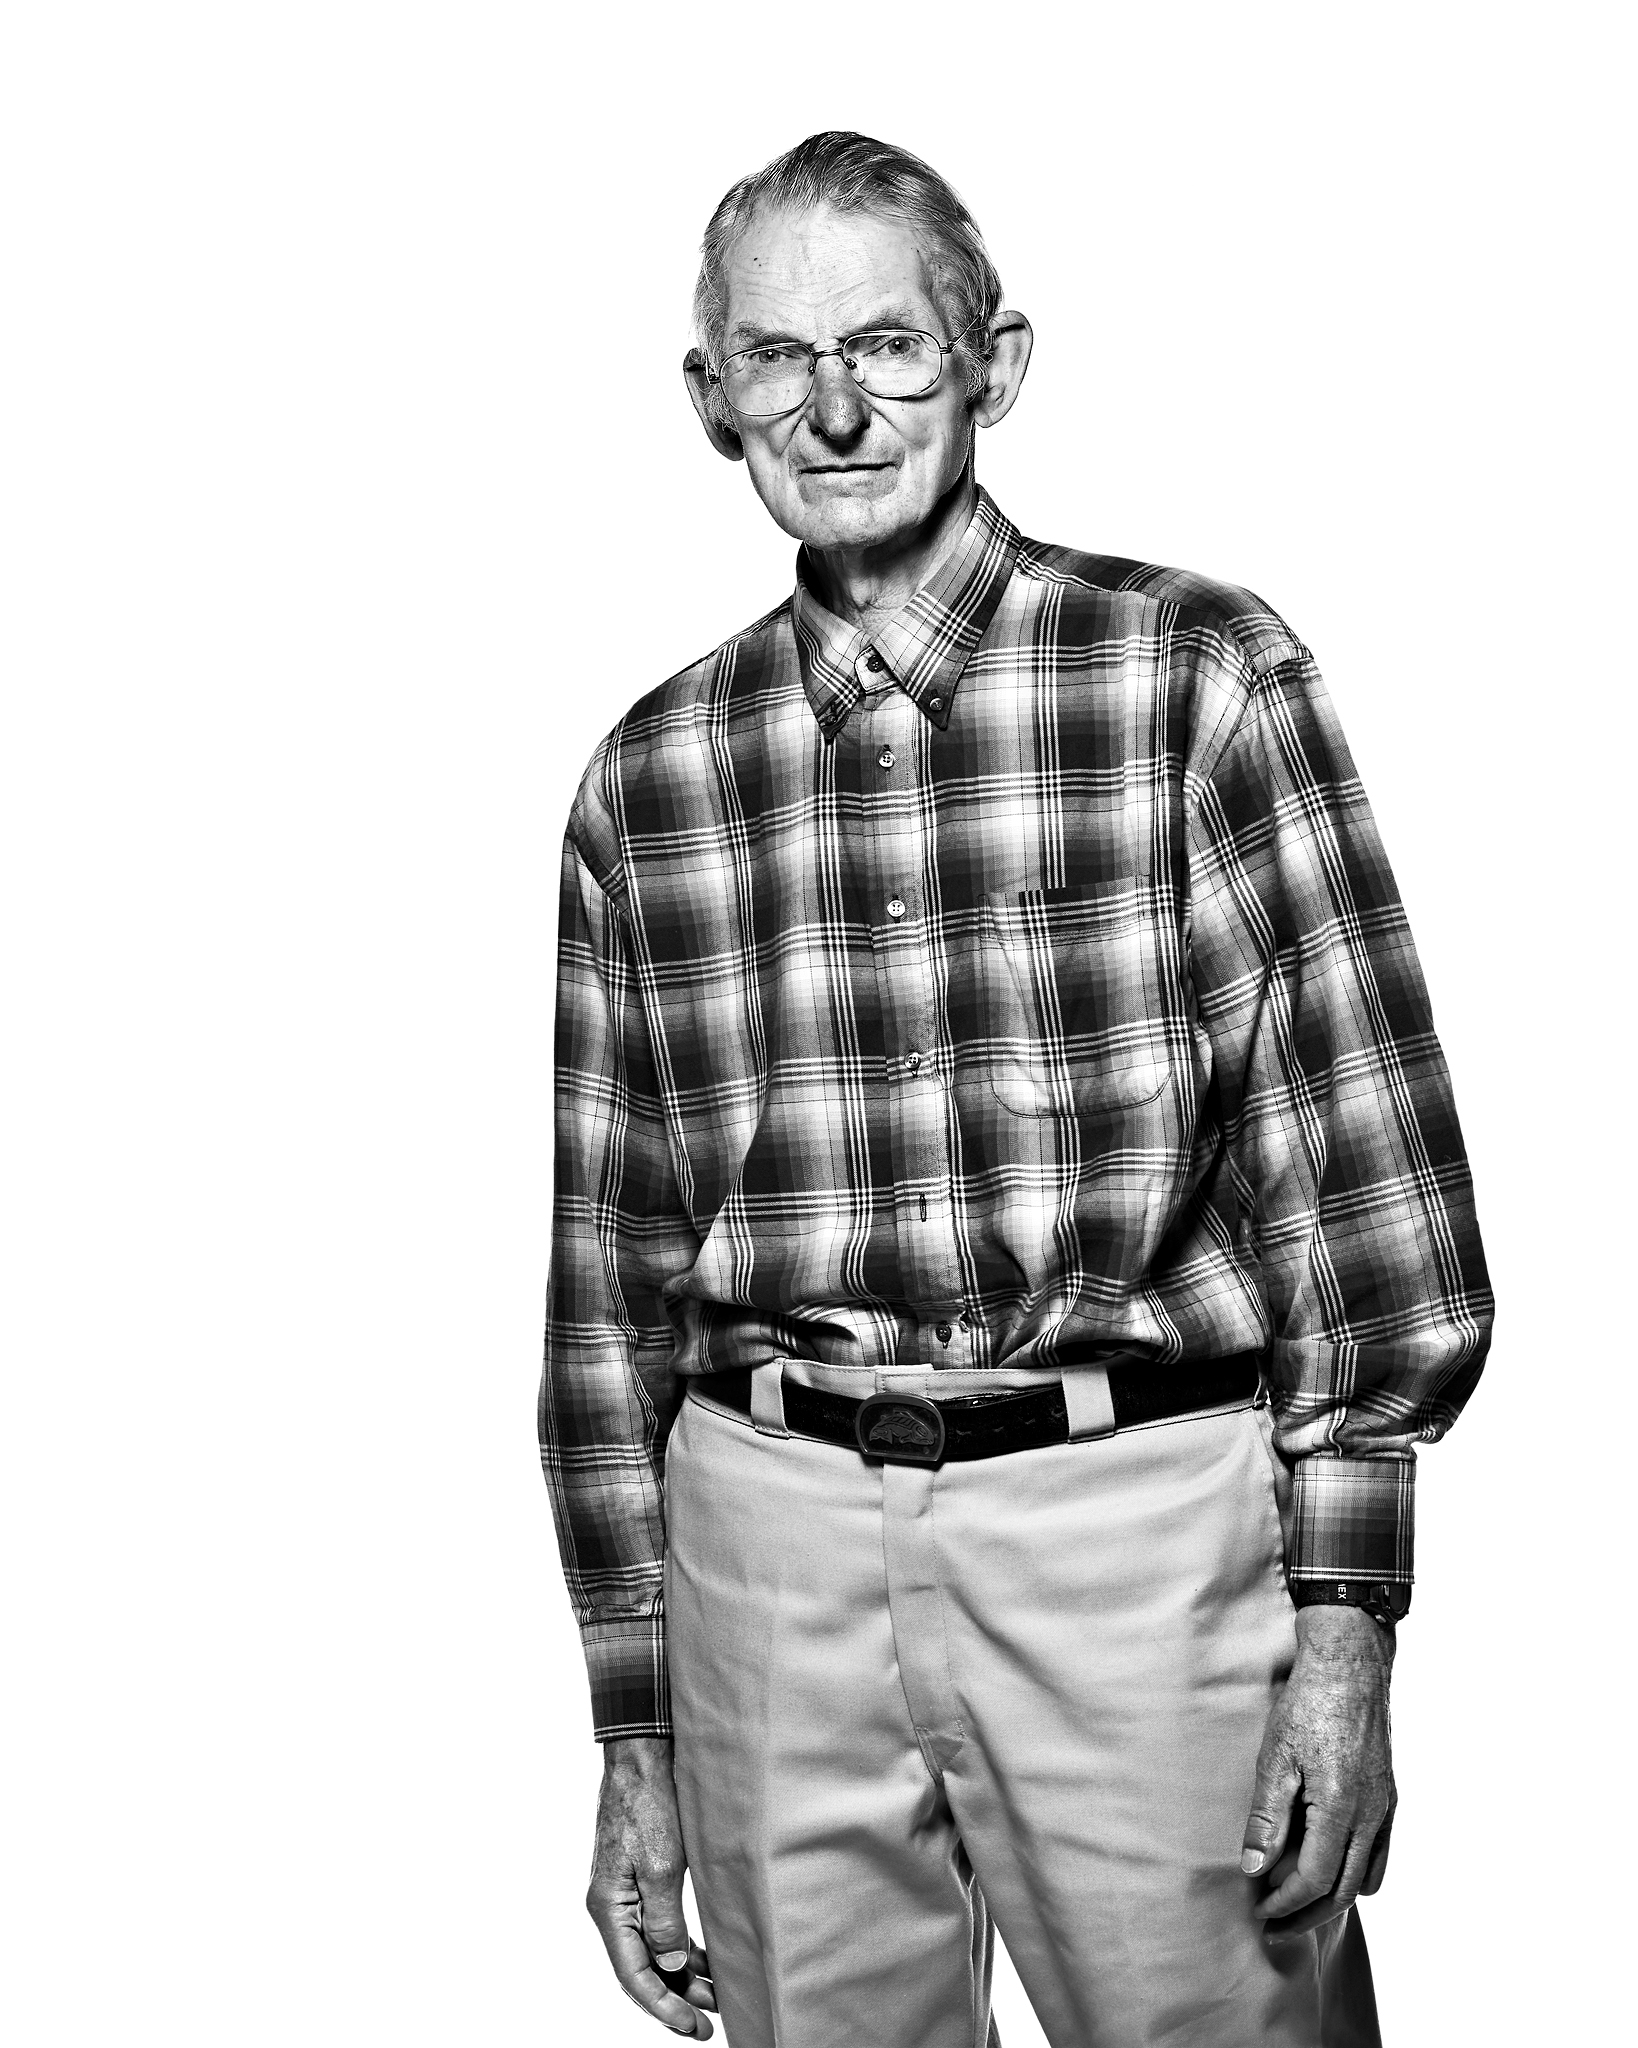
\includegraphics[height=5cm]{images/doug_mcilroy.jpg}
                \end{center}
        \end{column}
    \end{columns}
\end{frame}


\begin{frame}{Donald Knuth}
    \begin{columns}
        \begin{column}{0.6\textwidth}
            \begin{enumerate}
                \item Fundamental Algorithms
                \item Seminumerical Algorithms
                \item Sorting and Searching
                \item Combinatorial Algorithms
                \item Syntactic Algorithms
                \item The Theory of Context-free Languages
                \item Compiler Techniques
            \end{enumerate}
        \end{column}
        \begin{column}{0.4\textwidth}  %%<--- here
                \begin{center}
					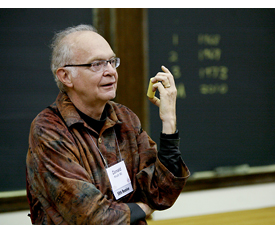
\includegraphics[height=3.5cm]{images/knuth.jpg}
                \end{center}
        \end{column}
    \end{columns}
\end{frame}

\begin{frame}{Niklaus Wirth}
    \begin{columns}
        \begin{column}{0.6\textwidth}
	        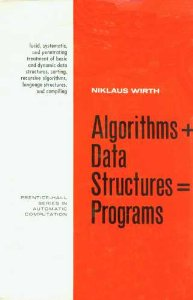
\includegraphics[height=7cm]{images/algorithms_data_structures_programs.jpg}
        \end{column}
        \begin{column}{0.4\textwidth}  %%<--- here
                \begin{center}
					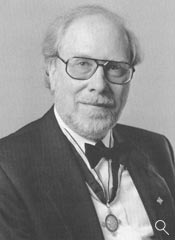
\includegraphics[height=5cm]{images/wirth.jpg}
                \end{center}
        \end{column}
    \end{columns}
\end{frame}

\begin{frame}{Edsger Wybe Dijkstra}
    \begin{columns}
        \begin{column}{0.6\textwidth}
            \begin{figure}
    	        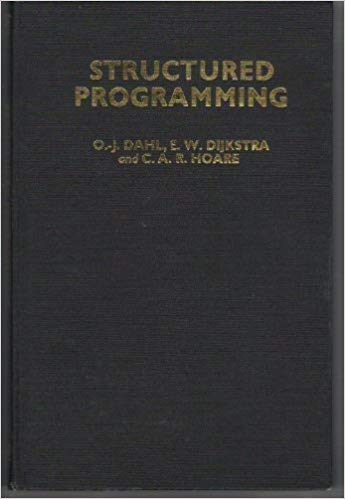
\includegraphics[height=6cm]{images/structured_programming.jpg}
	    	    \caption{We need structured programming}
            \end{figure}
        \end{column}
        \begin{column}{0.4\textwidth}  %%<--- here
                \begin{center}
					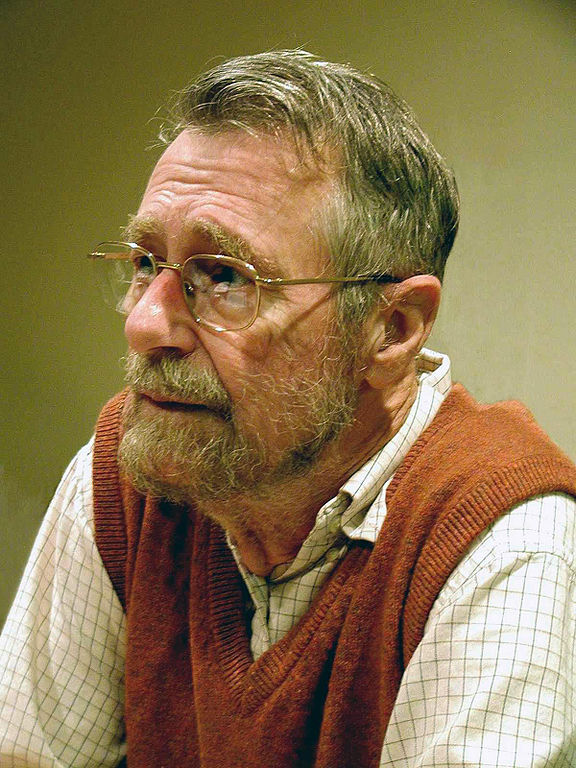
\includegraphics[height=5cm]{images/dijstra.jpg}
                \end{center}
        \end{column}
    \end{columns}
\end{frame}


\begin{frame}{John Backus}
    \begin{columns}
        \begin{column}{0.6\textwidth}
            \begin{figure}
    	        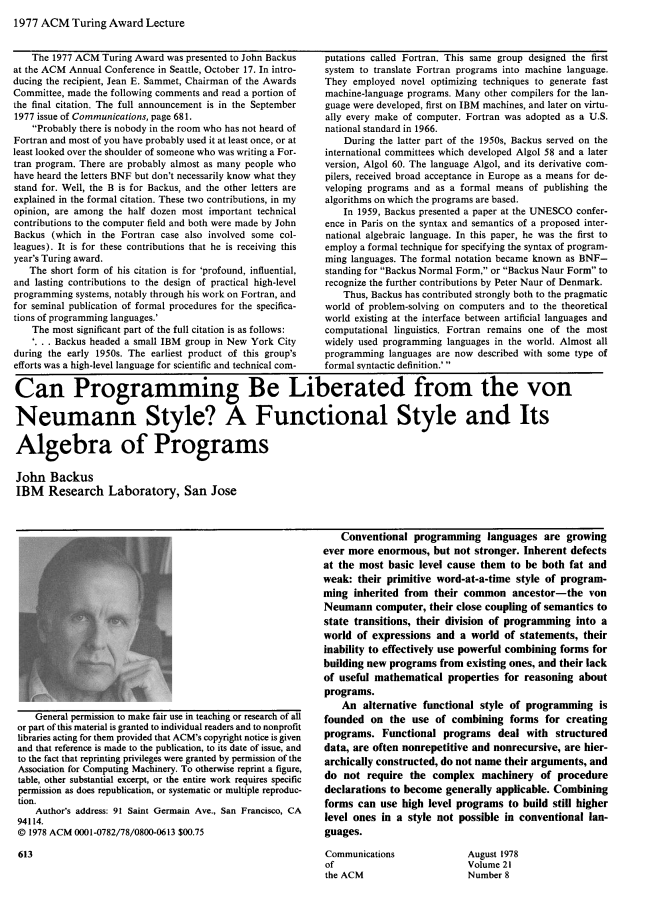
\includegraphics[height=6cm]{images/functional.png}
	    	    \caption{We need a few functional forms}
            \end{figure}
        \end{column}
        \begin{column}{0.4\textwidth}  %%<--- here
                \begin{center}
					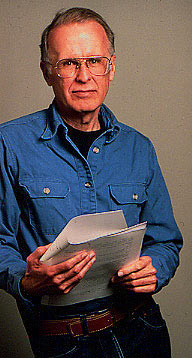
\includegraphics[height=5cm]{images/backus.jpg}
                \end{center}
        \end{column}
    \end{columns}
\end{frame}





\begin{frame}{Dmitri Mendeleev}
    \begin{columns}
        \begin{column}{0.6\textwidth}
			\begin{figure}
				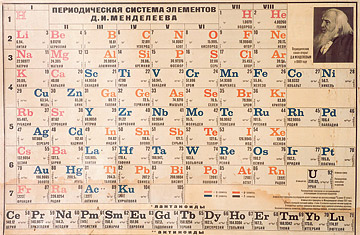
\includegraphics[height=4cm]{images/periodic_table.jpg}
				\caption{A Russian periodic table based on Dmitri Mendeleyev's original table of 1869.}
			\end{figure}
        \end{column}
        \begin{column}{0.4\textwidth}  %%<--- here
                \begin{center}
					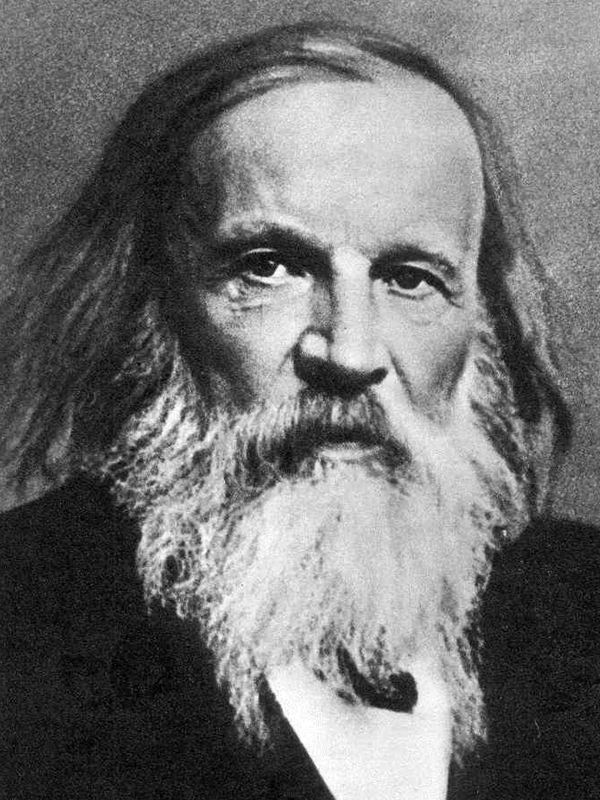
\includegraphics[height=5cm]{images/mendeleev.jpg}
                \end{center}
        \end{column}
    \end{columns}
\end{frame}



\begin{frame}{Carl Linnaeus}
    \begin{columns}
        \begin{column}{0.6\textwidth}
			Species Plantarum lists every species of plant known at the time, classified into genera. It is the first work to consistently apply binomial names and was the starting point for the naming of plants.
        \end{column}
        \begin{column}{0.4\textwidth}  %%<--- here
                \begin{center}
					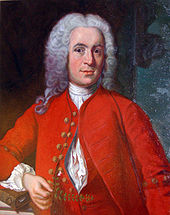
\includegraphics[height=5cm]{images/LinnaeusWeddingPortrait.jpg}
                \end{center}
        \end{column}
    \end{columns}
\end{frame}

\begin{frame}{Euclid}
	\begin{columns}
        \begin{column}{0.6\textwidth}
			\begin{enumerate}
				\item Definitions
				\item Postulates
				\item Common notions
			\end{enumerate}
		\end{column}
        \begin{column}{0.4\textwidth}  %%<--- here
                \begin{center}
					
\includegraphics[height=5cm]{images/euclid.jpg}
                \end{center}
        \end{column}
	\end{columns}
\end{frame}

\begin{frame}{Common Notions}
\begin{enumerate}
	\item Things which are equal to the same thing are also equal to one other.
	\item If equals be added to equals, the wholes are equal.
	\item If equals be subructed from equals, the remainders are equal.
	\item Things which coincide with one another are equal to one another.
	\item The whole is greater than the part.
\end{enumerate}
\end{frame}



\begin{frame}{Basic idea}
\begin{block}{}
The essence of generic programming lies in the idea of concepts. A concept is a way of describing a family of related object types.
\end{block}
\begin{center}
    \begin{tabular}{ | p{1.5cm} | l | l | p{3cm} |}
    \hline
    \textbf{Natural Science} & \textbf{Mathematics} & \textbf{Programming} & \textbf{Programming Examples} \\ \hline
      genus & theory & concept & Integral, Character \\ \hline
      species & model & type or class & uint8\_t, char \\ \hline
      individual & element & instance  & 01000001(65, 'A') \\
    \hline
    \end{tabular}
\end{center}
\end{frame}


\begin{frame}[fragile]{Definitions}
  \begin{enumerate}
    \item Datum
    \item Value
    \item Value type
    \item Object
    \item Object type
  \end{enumerate}
\end{frame}



\begin{frame}[fragile]{Datum}
\begin{block}{Definition}
A \textbf{datum} is a sequence of bits.
\end{block}

\begin{block}{Example}
01000001 is an example of a datum.
\end{block}

\end{frame}

\begin{frame}[fragile]{Value}
\begin{block}{Definition}
A \textbf{value is} a \textbf{datum} together with its interpretation.
\end{block}
\begin{block}{Example}
The \textbf{datum} 01000001 might have the interpretation of the integer 65, or the character “A".
\end{block}
\begin{block}{Explanation}
Every \textbf{value} must be associated with a \textbf{datum} in memory; there is no way to refer to disembodied \textbf{values} in modern programming languages.
\end{block}
\end{frame}

\begin{frame}[fragile]{Value type}
\begin{block}{Definition}
A \textbf{value type} is a set of values sharing a common interpretation.
\end{block}
\end{frame}

\begin{frame}[fragile]{Object}
\begin{block}{Definition}
An \textbf{object} is a collection of bits in memory that contain a \textbf{value} of a given \textbf{value type}.
\end{block}
\begin{block}{Explanation}
An \textbf{object} is immutable if the value never changes, and mutable otherwise. An object is unrestricted if it can contain any \textbf{value} of its \textbf{value type}.
\end{block}
\end{frame}


\begin{frame}[fragile]{Object type}
\begin{block}{Definition}
An \textbf{object type} is a uniform method of storing and retrieving \textbf{values} of a given \textbf{value type} from a particular \textbf{object} when given its address.
\end{block}
\end{frame}


\section{Journey}
\begin{frame}{How algorithms were selected?}
  \begin{enumerate}
    \item useful
    \item generic
    \item fits into 1 slide
  \end{enumerate}
\end{frame}


\begin{frame}{Semiregular}
    \begin{block}{Operation}
      \begin{enumerate}
        \item Copy construction
        \item Assignment
        \item Destruction
      \end{enumerate}
    \end{block}

    \begin{block}{Semantic}
        $$\forall a ~ \forall b ~ \forall c : T~a(b)  \implies(b = c \implies a = c)$$
        $$\forall a ~ \forall b ~ \forall c : a \leftarrow b  \implies(b = c \implies a = c)$$
        $$\forall f \in RegularFunction: a = b \implies f(a) = f(b)$$
    \end{block}
\end{frame}

\begin{frame}[fragile]{Semiregular}
\begin{lstlisting}[style=cpp]

template<typename T>
concept semiregular = std::is_default_constructible<T>::value &&
                      std::is_copy_constructible<T>::value &&
                      std::is_copy_assignable<T>::value &&
                      std::is_destructible<T>::value

\end{lstlisting}
\end{frame}

\begin{frame}{Regular type}
\begin{block}{Operation}
  \begin{enumerate}
    \item Copy construction
    \item Assignment
    \item Equality
    \item Destruction
  \end{enumerate}
\end{block}
\begin{block}{Semantic}
    $$\forall a ~ \forall b ~ \forall c : T~a(b)  \implies(b = c \implies a = c)$$
    $$\forall a ~ \forall b ~ \forall c : a \leftarrow b  \implies(b = c \implies a = c)$$
    $$\forall f \in RegularFunction: a = b \implies f(a) = f(b)$$
\end{block}
\end{frame}

\begin{frame}[fragile]{Regular}
\begin{lstlisting}[style=cpp]

template<typename T>
concept semiregular = semiregular<T> && is_equality_comparable<T>::value;

\end{lstlisting}
\end{frame}

\begin{frame}{Relation}
    \begin{align*}
        FunctionalProcedure(F) \triangleq F~is~a~regular~procedure~defined~on~regular~&\\
        types:~replacing~its~inputs~with~equal~objects~\\
        results~in~equal~output~objects. \\\\
        UnaryFunction(F) \triangleq FunctionalProcedure(F) \land Arity(F) = 1 &\\
                \land~Domain: UnaryFunction \rightarrow Regular &\\
                F \mapsto InputType(F, 0)\\\\
        HomogeneousFunction(F) \triangleq FunctionalProcedure(F) \land Arity(F) > 0\\
        \land (\forall i,j \in \mathbb{N})(i,j < Arity(F)) \implies (InputType(F, i) = InputType(F, j))\\
        \land Domain: HomogeneousFunction \rightarrow Regular\\
        F \implies InputType(F, 0)
    \end{align*}
\end{frame}



\begin{frame}[fragile]{Regular}
\begin{lstlisting}[style=cpp]
template<typename F, typename... T>
concept functional_procedure = (regular<typename std::invoke_result<F, T...>::type> || std::is_same<typename std::invoke_result<F, T...>::type, void>::value) && is_regular<T...>::value;

template<typename F, typename T>
concept unary_function = functional_procedure<F, T> && regular<T>;

template<typename F, typename... T>
concept homogeneous_function = functional_procedure<F, T...> && sizeof...(T) > 0 && all_same<T...>::value && all_regular<T>;

\end{lstlisting}
\end{frame}



\begin{frame}
\begin{align*}
    Predicate(P) \triangleq FunctionalProcedure(F) \land Codomain(P) = bool\\\\
    HomogeneousPredicate(P) \triangleq Predicate(P) \land HomogeneousFunction(P) \\\\
    Relation(R) \triangleq HomogeneousPredicate(R) \land Arity(R) = 2\\\\
\end{align*}

\end{frame}


\begin{frame}[fragile]{Relation}
\begin{lstlisting}[style=cpp]
template<typename F, typename... T>
concept predicate = functional_procedure<F, T...> && std::is_same<codomain_t<F, T...>, bool>::value;

template<typename F, typename... T>
concept homogeneous_predicate = predicate<F, T...> && homogeneous_function<F, T...>;

template<typename R, typename T>
concept relation = predicate<R, T, T>;
\end{lstlisting}
\end{frame}


\begin{frame}{Totally Ordered}
    \begin{align*}
        property(R: Relation)\\
        transitive: R \\
                r \mapsto (\forall a,b,c \in Domain(R)) (r(a, b) \land r(b,c) \implies r(a, c))\\\\
        property(R: Relation)\\
        total\_ordering: R \\
                r \mapsto transitive(r)~\land(\forall a,b \in Domain(R))~exactly~one~of~following~holds:\\
            r(a, b),~r(b, a),~or~a = b\\
    \end{align*}

    \begin{align*}
        TotallyOrdered(T) \triangleq Regular(T) \land <: T~x~T \rightarrow bool \land total\_ordering(<)
    \end{align*}
\end{frame}

\begin{frame}[fragile]{Totally Ordered}
\begin{lstlisting}[style=cpp]
template<typename T>
concept totally_ordered = regular<T> && is_less_than_comprable<T>::value;

\end{lstlisting}
\end{frame}


\begin{frame}{Journey 1}
    \begin{enumerate}
        \item min
        \item max
    \end{enumerate}
\end{frame}

\begin{frame}{Journey \#1}
    \begin{block}{}
		\lstinputlisting[style=cpp]{code/snippets/1/0.min.0.h}
	\end{block}
\end{frame}

\begin{frame}{Journey \#1}
    \begin{block}{}
		\lstinputlisting[style=cpp]{code/snippets/1/0.min.1.h}
	\end{block}
\end{frame}


\begin{frame}{Journey \#1}
    \begin{block}{}
		\lstinputlisting[style=cpp]{code/snippets/1/0.min.2.h}
	\end{block}
\end{frame}

\begin{frame}{Journey \#1}
    \begin{block}{Dealing with large objects}
		\lstinputlisting[style=cpp]{code/snippets/1/0.min.3.h}
	\end{block}
\end{frame}

\begin{frame}{Journey \#1}
    \begin{block}{}
		\lstinputlisting[style=cpp]{code/snippets/1/0.min.4.h}
	\end{block}
\end{frame}

\begin{frame}{Journey \#1}
    \begin{block}{}
		\lstinputlisting[style=cpp]{code/snippets/1/0.min.5.cpp}
	\end{block}
\end{frame}

\begin{frame}{Journey \#1}
    \begin{block}{}
		\lstinputlisting[style=cpp]{code/snippets/1/0.min.6.h}
	\end{block}
\end{frame}

\begin{frame}[fragile]{Journey \#1}
\begin{lstlisting}[style=cpp]

template<totally_ordered T>
const T& min(const T& x, const T& y) {
    if (y < x) {
        return y;
    }
    return x;
}


template<totally_ordered T>
T& min(T& x, T& y) {
    if (y < x) {
        return y;
    }
    return x;
}

\end{lstlisting}
\end{frame}


\begin{frame}[fragile]{Journey \#1}
\begin{lstlisting}[style=cpp]
template<typename T, weak_strict_ordering<T> R>
const T& min(const T& x, const T& y, R r) {
    if (r(y, x)) {
        return y;
    }
    return x;
}

template<typename T, weak_strict_ordering<T> R>
T& min(T& x, T& y, R r) {
    if (r(y, x)) {
        return y;
    }
    return x;
}
\end{lstlisting}
\end{frame}

\begin{frame}[fragile]{Journey \#1}
\begin{lstlisting}[style=cpp]
template<typename T, unary_function<T> Projection>
requires totally_ordered<codomain_t<Projection, T>>
const T& min(const T& x, const T& y, Projection projection) {
    if (projection(y) < projection(x)) {
        return y;
    }
    return x;
}


template<typename T, unary_function<T> Projection>
requires totally_ordered<codomain_t<Projection, T>>
T& min(T& x, T& y, Projection projection) {
    if (projection(y) < projection(x)) {
        return y;
    }
    return x;
}

\end{lstlisting}
\end{frame}





\begin{frame}[fragile]{Journey \#1}
\begin{lstlisting}[style=cpp]

template<totally_ordered T>
const T& max(const T& x, const T& y) {
    if (y < x) {
        return x;
    }
    return y;
}


template<totally_ordered T>
T& max(T& x, T& y) {
    if (y < x) {
        return x;
    }
    return y;
}

\end{lstlisting}
\end{frame}

\begin{frame}{Journey \#2}
    \begin{enumerate}
        \item unique\_count
        \item unique\_copy
        \item unique
    \end{enumerate}
\end{frame}

\begin{frame}{Journey \#2. Intuinition behind unique\_count and unique\_copy}
    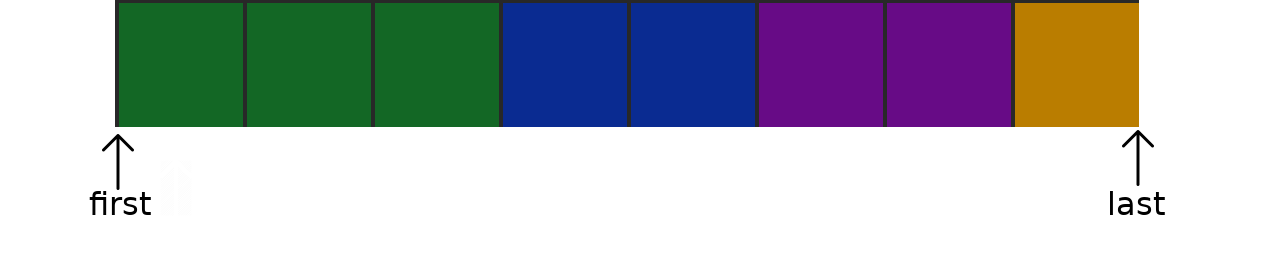
\includegraphics[height=2cm]{images/sequence.png}
    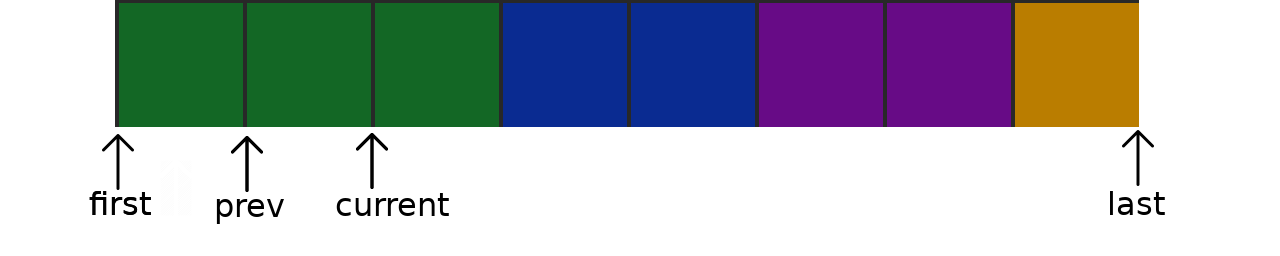
\includegraphics[height=2cm]{images/sequence2.png}
    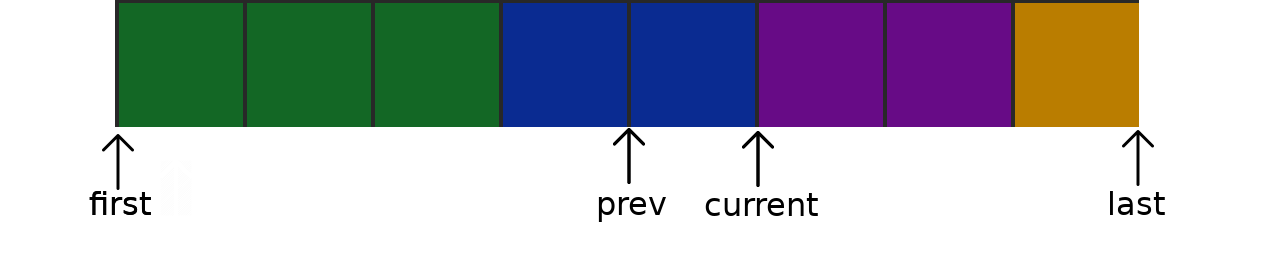
\includegraphics[height=2cm]{images/sequence3.png}
\end{frame}

\begin{frame}{Journey \#2. Intuinition behind unique}
    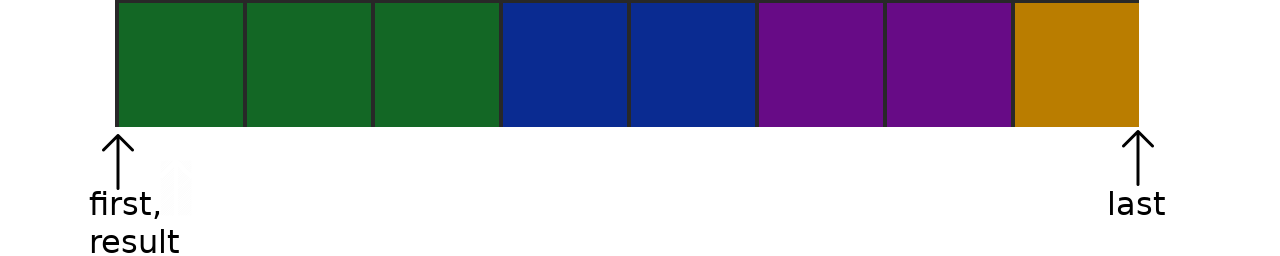
\includegraphics[height=2cm]{images/sequence-1-3-1.png}
    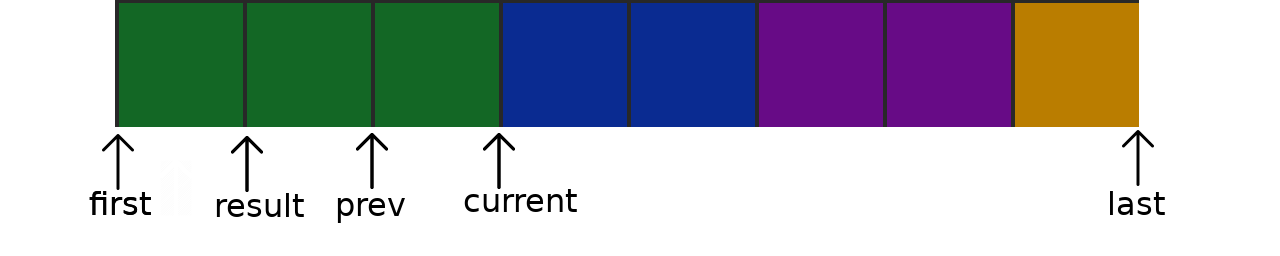
\includegraphics[height=2cm]{images/sequence-1-3-2.png}
    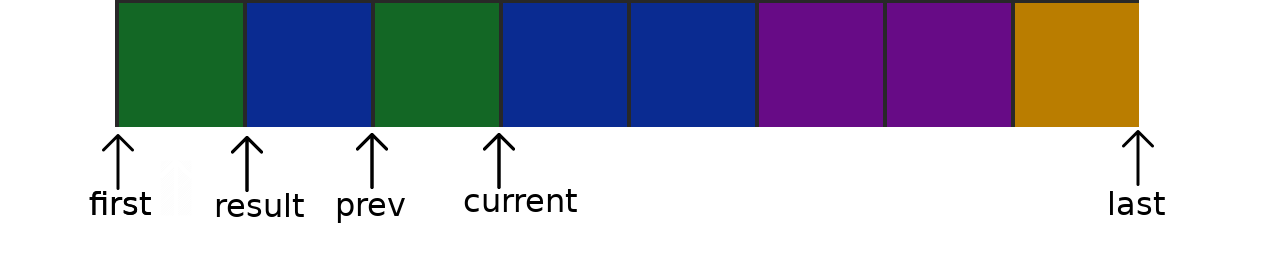
\includegraphics[height=2cm]{images/sequence-1-3-3.png}
\end{frame}



\begin{frame}{Concepts}
    \begin{align*}
        Iterator(T) ~\triangleq~ & Regular(T) ~\land \\
        & DistanceType: Iterator \rightarrow Integer ~\land \\
        & successor: T \rightarrow T ~\land\\
        & successor~is~not~necessarily-regular\\\\
        ForwardIterator(T) ~\triangleq~ & Iterator(T) ~\land ~regular\_unary\_function(successor)
    \end{align*}
\end{frame}


\begin{frame}[fragile]{Concepts}
\begin{lstlisting}[style=cpp]
template<typename I>
concept iterator = std::is_same<std::forward_iterator_tag, typename std::iterator_traits<I>::iterator_category>::value ||
                   std::is_same<std::input_iterator_tag, typename std::iterator_traits<I>::iterator_category>::value ||
                   std::is_same<std::output_iterator_tag, typename std::iterator_traits<I>::iterator_category>::value ||
                   std::is_same<std::bidirectional_iterator_tag, typename std::iterator_traits<I>::iterator_category>::value ||
                   std::is_same<std::random_access_iterator_tag, typename std::iterator_traits<I>::iterator_category>::value;

template<typename I>
concept forward_iterator = iterator<I> && std::is_base_of<std::forward_iterator_tag, typename std::iterator_traits<I>::iterator_category>::value;
\end{lstlisting}
\end{frame}

\begin{frame}{Concepts}
    \begin{align*}
        BidirectionalIterator(T) ~\triangleq~ & ForwardIterator(T) ~\land \\
                                              & predecessor: T \rightarrow T ~\land \\
                                              & predecessor~takes~constant~type ~\land \\
                                              & (\forall i \in T) successor(i) is defined~\implies \\
                                              & ~~~~predecessor(successor(i))~is~defined \\
                                              & ~~~~and~equals~to~i~ \land\\
                                              & (\forall i \in T) predecessor(i)~is~defined~ \implies \\
                                              & ~~~~successor(predecessor(i))~is~defined\\
                                              & ~~~~and~equals~to~i
    \end{align*}
\end{frame}


\begin{frame}[fragile]{Concepts. Bidirectioanal Iterator}
\begin{lstlisting}[style=cpp]

template<typename I>
concept bidirectional_iterator = iterator<I> && std::is_base_of<std::bidirectional_iterator_tag, typename std::iterator_traits<I>::iterator_category>::value;

\end{lstlisting}
\end{frame}


\begin{frame}{Concepts. Indexed Iterator.}
    \begin{align*}
        IndexedIterator(T) ~\triangleq~ & ForwardIterator(T) ~\land \\
                                              & +: T~x~DifferenceType(T) \rightarrow T ~\land\\
                                              & -: T~x~T \rightarrow DifferenceType(T) ~\land\\
                                              & + takes~constant~time\\
                                              & - takes~constant~time
    \end{align*}
\end{frame}



\begin{frame}{Concepts. Random Access Iterator}
    \begin{align*}
        RandomAccessIterator(T)  ~\triangleq~ & BidirectionalIterator(T) ~\land \\
                                              & IndexedIterator(T) ~\land \\
                                              & TotallyOrdered(T) ~\land \\
                                              & (\forall i,j \in T) ~i < j \iff i \prec j ~ \land \\
                                              & DifferenceType: \\
                                              & ~~~~RandomAccessIterator \rightarrow Integer ~ \land\\
                                              & +: T~x~DifferenceType(T) \rightarrow T ~\land\\
                                              & -: T~x~DifferenceType(T) \rightarrow T ~\land\\
                                              & -: T~x~T \rightarrow DifferenceType(T) ~\land\\
                                              & < takes~constant~time ~\land\\
                                              & - between~and~iterator~and~an~integer \\
                                              & ~~~~takes~constant~time
    \end{align*}
\end{frame}

\begin{frame}[fragile]{Concepts. Random Access Iterator Iterator}
\begin{lstlisting}[style=cpp]

template<typename I>
concept random_access_iterator= iterator<I> && std::is_base_of<std::random_access_iterator_tag, typename std::iterator_traits<I>::iterator_category>::value;

\end{lstlisting}
\end{frame}

\begin{frame}{Concepts. Readable}
    \begin{align*}
        Readable(T) ~\triangleq~ & Regular(T) ~\land \\
        & ValueType: Readable \rightarrow Regular ~\land \\
        & source: T \rightarrow ValueType(T)
    \end{align*}
\end{frame}

\begin{frame}[fragile]{Concepts. Readable}
\begin{lstlisting}[style=cpp]
template<typename T>s
concept readable = std::is_same<decltype(*std::declval<T>()), value_type_t<T>&>::value || std::is_same<decltype(*std::declval<T>()), const value_type_t<T>&>::value;
\end{lstlisting}
\end{frame}

\begin{frame}{Concepts. Writable}
    \begin{align*}
        Writable(T) ~\triangleq~ & ValueType: Writable \rightarrow Regular ~\land \\
        & (\forall x \in T) (\forall v \in ValueType(T))~sink(x)~\leftarrow~v ~ \\
        & ~~~~is~a~well-formed~statement
        %& source: T \rightarrow ValueType(T) ~\land\\
    \end{align*}
\end{frame}

\begin{frame}[fragile]{Concept: writable}
\begin{lstlisting}[style=cpp]
template<typename T, typename U = ValueType(T)>
concept writable = requires(T it, U x) { *it = x; }; 
\end{lstlisting}
\end{frame}

\begin{frame}[fragile]{Concept: writable}
\begin{lstlisting}[style=cpp]

template<typename T>
concept additive_semigroup = regular<T> && std::is_same<decltype(T() + T()), T>::value; 

template<typename T>
concept additive_monoid = additive_semigroup<T>; // 0 \in T, identity_element(T);

\end{lstlisting}
\end{frame}

\begin{frame}[fragile]{unique\_count}
\begin{lstlisting}[style=cpp]
N unique_count(It first, It last, N n, R r) {
    if (first == last) { return n; }
    // some algorithm
    return n;
}

\end{lstlisting}
\end{frame}

\begin{frame}[fragile]{unique\_count}
\begin{lstlisting}[style=cpp]
N unique_count(It first, It last, N n, R r) {
    if (first == last) { return n; }
    It previous = first;
    ++first;
    // some algorithm
    return n;
}

\end{lstlisting}
\end{frame}

\begin{frame}[fragile]{unique\_count}
\begin{lstlisting}[style=cpp]
N unique_count(It first, It last, N n, R r) {
    if (first == last) { return n; }
    It previous = first;
    ++first;
    ++n;

        if (!r(*previous, *first)) {
            ++n;
        }
        
    return n;
}

\end{lstlisting}
\end{frame}


\begin{frame}[fragile]{unique\_count}
\begin{lstlisting}[style=cpp]
N unique_count(It first, It last, N n, R r) {
    if (first == last) { return n; }
    It previous = first;
    ++first;
    while (first != last) {
        if (!r(*previous, *first)) {
            ++n;
        }
       ++previous;
       ++first;
    }
    ++n;
    return n;
}

\end{lstlisting}
\end{frame}



\begin{frame}[fragile]{unique\_count}
\begin{lstlisting}[style=cpp]
template<forward_iterator It, additive_monoid N, relation<value_type_t<It>> R>
N unique_count(It first, It last, N n, R r) {
    if (first == last) { return n; }
    It previous = first;
    ++first;
    while (first != last) {
        if (!r(*previous, *first)) {
            ++n;
        }
       ++previous;
       ++first;
    }
    ++n;
    return n;
}

\end{lstlisting}
\end{frame}


\begin{frame}[fragile]{unique\_count}
\begin{lstlisting}[style=cpp]
template<forward_iterator It, additive_monoid N>
requires(readable<It>)
N unique_count(It first, It last, N n) {
    return unique_count(first, last, n, std::equal_to<value_type_t<It, It>());
}
\end{lstlisting}
\end{frame}

\begin{frame}[fragile]{unique\_copy}
\begin{lstlisting}[style=cpp]

template<forward_iterator It, output_iterator Out, relation<value_type_t<It>> R>
requires readable<It> && writable<Out, value_type_t<It>>
Out unique_copy(It first, It last, Out out, R r) {
    if (first == last) { return out; }
    *out = *first;  
    ++out;
    It previous = first; ++first;
    while (first != last) {
        if (!r(*previous, *first)) {
          *out = *first;
          ++out;
        }
        ++first;
        ++previous;
    }
    return out;
}

\end{lstlisting}
\end{frame}

\begin{frame}[fragile]{unique\_copy}
\begin{lstlisting}[style=cpp]

template<forward_iterator It, output_iterator Out>
requires readable<It> && writable<Out, value_type_t<It>>
Out unique_copy(It first, It last, Out out) {
    return cppcon::unique_copy(first, last, out, std::equal_to<value_type_t<It>>());
}

\end{lstlisting}
\end{frame}

\begin{frame}[fragile]{unique}
\begin{lstlisting}[style=cpp]
template<forward_iterator It, relation<value_type_t<It>> R>
requires readable<It> && writable<It>
It unique(It first, It last, R r) {
    if (first == last) { return last; }
    It result = first; ++first;
    while (first != last) {
        if (r(*result, *first)) {
           ++first;
        } else {
            ++result;
            *result = *first;
            ++first;
        }
    }
    ++result;
    return result;
}

\end{lstlisting}
\end{frame}


\begin{frame}[fragile]{Journey \#2. unique}
    \begin{lstlisting}[style=cpp]
    template<forward_iterator It>
    requires(regular<value_type_t<It>> && readable<It> && writable<It>)
    It unique(It first, It last) {
        return cppcon::unique(first, last, std::equal_to<value_type_t<It>>());
    }
    \end{lstlisting}
\end{frame}

\begin{frame}{Journey \#3}
    \begin{enumerate}
        \item frequencies 
        \item transform\_subgroups
        \item squash\_subgroups
    \end{enumerate}
\end{frame}


\begin{frame}[fragile]{Journey \#3. frequencies}
\begin{lstlisting}[style=cpp]

template<forward_iterator It, output_iterator Out>
requires readable<It> && writable<Out, std::pair<value_type_t<It>, size_t>>
Out frequencies(It f, It l, Out out) {
  typedef size_t N;
  while (f != l) { 
    It it = f;
    N n = 1;
    ++f;
    auto r = find_not(f, l, *it, n);
    f = r.first;
    *out = { *it, r.second };
    ++out;
  } 
  return out;
}

\end{lstlisting}
\end{frame}


\begin{frame}[fragile]{Journey \#3. frequencies}
\begin{lstlisting}[style=cpp]

template<forward_iterator It, output_iterator Out, relation<value_type_t<It>> R>
requires readable<It> && writable<Out, std::pair<value_type_t<It>, size_t>>
Out frequencies(It f, It l, Out out, R r) {
  typedef size_t N;
  while (f != l) { 
    It start = f;
    N n = 1;
    ++f;
    auto r = find_if_not(f, l, *start, r, n);
    f = r.first;
    *out = { *start, r.second };
    ++out;
  } 
  return out;
}

\end{lstlisting}
\end{frame}


\begin{frame}[fragile]{Journey \#3. Frequencies}
\begin{lstlisting}[style=cpp]

template<forward_iterator It, output_iterator Out0, output_iterator Out1>
requires readable<It> && writable<Out0, value_type_t<It>> && writable<Out1, size_t>
std::pair<Out0, Out1> frequencies(It f, It l, Out0 out0, Out1 out1) {
  typedef size_t N;

  while (f != l) { 
    It start = f;
    N n = 1;
    ++f;
    auto r = find_not(f, l, *start, n);

    *out0 = *start;
    ++out0;

    *out1 = r.second;
    ++out1;

    f = r.first;
  } 
  return {out0, out1};
}

\end{lstlisting}
\end{frame}

\begin{frame}[fragile]{Journey \# 3. Frequencies}
\begin{lstlisting}[style=cpp]

template<forward_iterator It, output_iterator Out0, forward_iterator Out1>
requires readable<It> && writable<Out0> && writable<Out1>
std::pair<Out0, Out1> frequencies(It f, It l, Out0 out0, Out1 out1) {
  typedef value_type_t<Out1> N;

  while (f != l) { 
    It it = f;
    N n = 1;
    ++f;
    It r = find_not(f, l, *it, n);

    *out0 = *it;
    ++out0;

    *out1 = r.second;
    ++out1;

    f = r.first;
  } 
  return {out0, out1};
}

\end{lstlisting}
\end{frame}


\begin{frame}[fragile]{Journey \# 3. Transform subgroups}
\begin{lstlisting}[style=cpp]

template<forward_iterator It,
         output_iterator Out,
         relation<value_type_t<It>> P,
         functional_procedure<It, It> F>
requires readable<It> && writable<Out, codomain_t<F, It, It>> 
Out transform_subgroups(It first, It last, Out out, P pred, F function) {
    if (first == last) { return out; }
    It previous = first;
    It fast = previous;
    ++fast;
    while (fast != last) {
        if (!pred(*previous, *fast)) {
            *out = function(first, fast);
            ++out;
            first = fast;
        }
        ++previous; ++fast;
    }
    *out = function(first, fast);
    return ++out;
}

\end{lstlisting}
\end{frame}


\begin{frame}[fragile]{Semiregular}
\begin{lstlisting}[style=cpp]

template<forward_iterator It,
         output_iterator Out,
         relation<value_type_t<It>> P,
         functional_procedure<It, distance_type_t<It>> F>
requires readable<It> && writable<Out, codomain_t<F, It, distance_type_t<It>> >
Out transform_subgroups(It first, It last, Out out, P pred, F function) {
    if (first == last) { return out; }
    It previous = first;
    It fast = previous;
    ++fast;
    distance_type_t<It> n = 0;
    while (fast != last) {
        if (!pred(*previous, *fast)) {
            *out = function(first, n);
            n = 0;
            ++out;
            first = fast;
        }
        ++n;
        ++previous; ++fast;
    }
    *out = function(first, n);
    return ++out;
}

\end{lstlisting}
\end{frame}



\begin{frame}[fragile]{Journey \# 3. Squash subgroups}
\begin{lstlisting}[style=cpp]

template<forward_iterator It,
         output_iterator Out,
         relation<value_type_t<It>> Predicate,
         functional_procedure<It, It> F>
requires readable<It> && writable<Out, codomain_t<F, It, distance_type_t<It>>>
Out squash_subgroups(It first, It last, Predicate pred, F function) {
    return transform_subgroups(first, last, first, pred, function);
}

\end{lstlisting}
\end{frame}

\begin{frame}{Journey \#4. split}
    \begin{enumerate}
        \item split
        \item transform\_splits
    \end{enumerate}
\end{frame}


\begin{frame}{Journey \#4. Intuinition behind efficient split}
    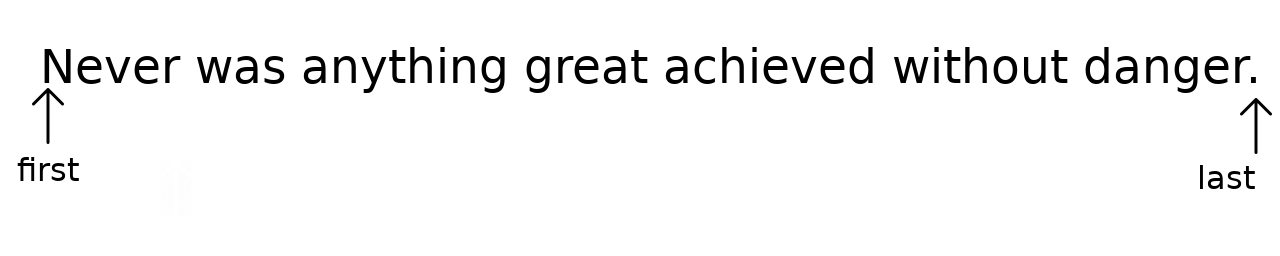
\includegraphics[height=2cm]{images/split-1.png}
    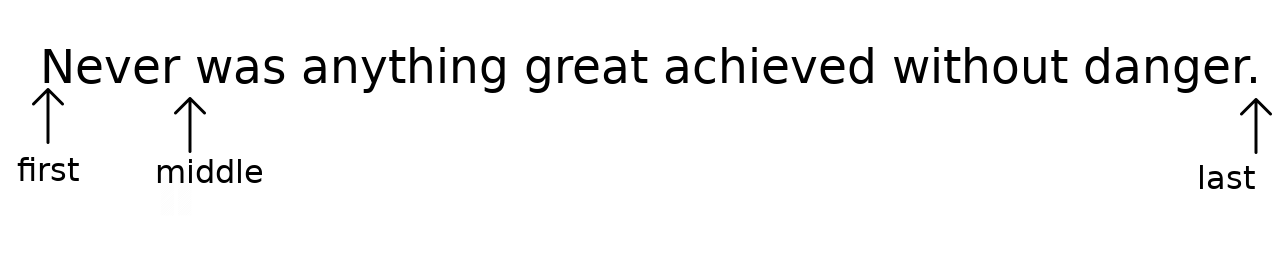
\includegraphics[height=2cm]{images/split-2.png}
    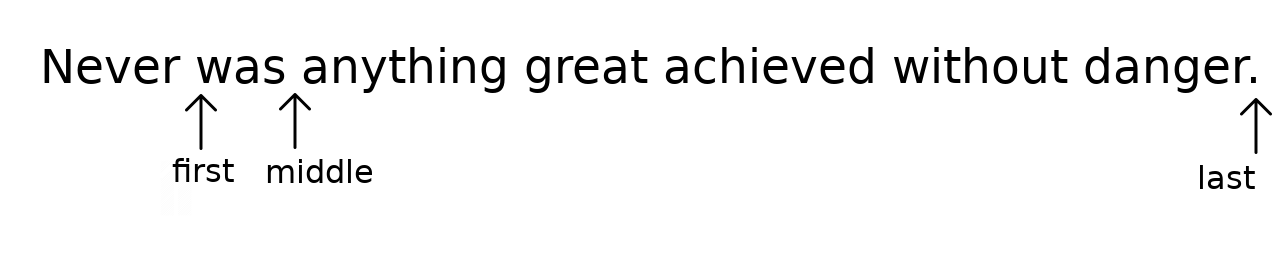
\includegraphics[height=2cm]{images/split-3.png}
\end{frame}


\begin{frame}[fragile]{Journey \# 4. Split}
\begin{lstlisting}[style=cpp]

template<forward_iterator It0, forward_iterator It1, functional_procedure<It0, It0> F>
requires readable<It0> && readable<It1>
void split(It0 first0, It0 last0, It1 first1, It1 last1, F f) {
    while (first0 != last0) {
        It0 middle = std::search(first0, last0, first1, last1);
        f(first0, middle);
        first0 = middle;
        if (first0 != last0) {
            ++first0;
        }
    }
}

\end{lstlisting}
\end{frame}


\begin{frame}[fragile]{Journey \# 4. Transform split}
\begin{lstlisting}[style=cpp]%%%%%%%

template<forward_iterator It0, output_iterator Out, forward_iterator It1, functional_procedure<It0, It0> F>
requires readable<It0> && readable<It1> && writable<Out, codomain_t<F, It0, It0>>
Out transform_split(It0 first0, It0 last0, Out out, It1 first1, It1 last1, F f) {
    auto step_size = std::distance(first1, last1);
    while (first0 != last0) {
        It0 middle = std::search(first0, last0, first1, last1);
        *out = f(first0, middle);
        ++out;
        first0 = middle;
        if (first0 != last0) {
            std::advance(first0, step_size);
        }
    }
    return out;
}

\end{lstlisting}
\end{frame}



\begin{frame}{Journey \#5}
    \begin{enumerate}
        \item remove
        \item remove\_if
        \item partition\_semistable
    \end{enumerate}
\end{frame}

\begin{frame}{Journey \#5. Intuinition behind the scene}
    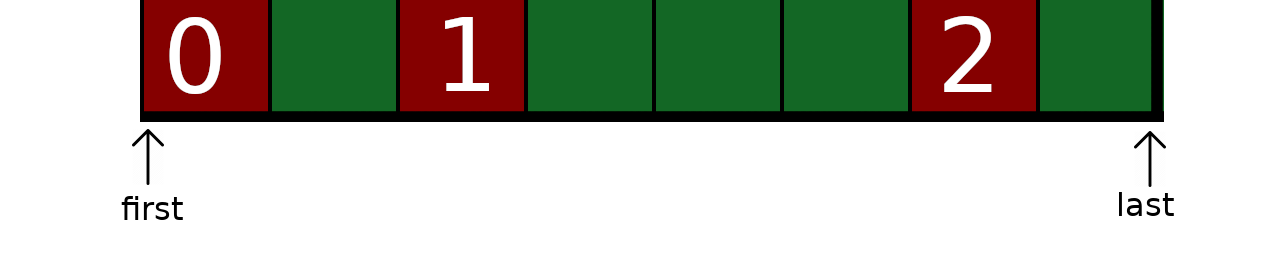
\includegraphics[height=2cm]{images/partition-1.png}
    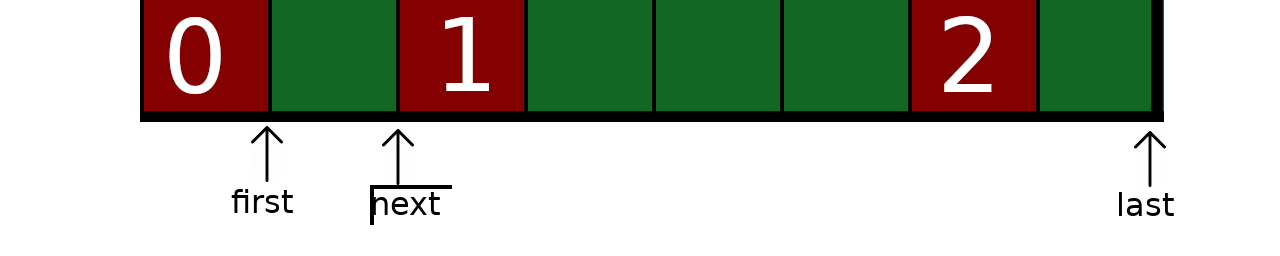
\includegraphics[height=2cm]{images/partition-2.png}
    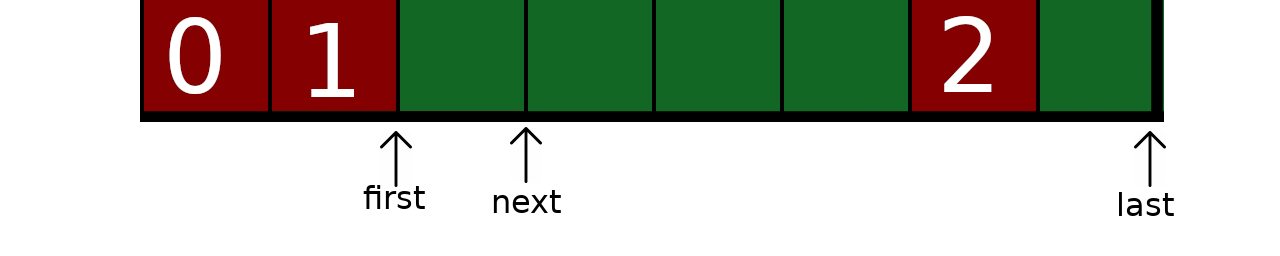
\includegraphics[height=2cm]{images/partition-3.png}
\end{frame}




\begin{frame}[fragile]{Journey \# 5. Remove}
\begin{lstlisting}[style=cpp] %%%%%%%

template<forward_iterator It>
requires readable<It> && writable<It>
It remove(It first, It last, const value_type_t<It>& value) {
    first = std::find(first, last, value);
    if (first == last) { return last; }
    It fast = first; ++fast;
    while (fast != last) {
        if (*fast == value) {
            ++fast;
        } else {
            *first = std::move(*fast);
            ++first; ++fast;
        }
    }
    return first;
}

\end{lstlisting}
\end{frame}


\begin{frame}[fragile]{Journey \# 5. Remove if}
\begin{lstlisting}[style=cpp] %%%%%%%

template<forward_iterator It, unary_predicate<value_type_t<It>> P>
requires readable<It> && writable<It>
It remove_if(It first, It last, P pred) {
    first = std::find_if(first, last, pred);
    if (first == last) { return last; }
    It fast = first; ++fast;
    while (fast != last) {
        if (pred(*fast)) {
            ++fast;
        } else {
            *first = std::move(*fast);
            ++first; ++fast;
        }
    }
    return first;
}

\end{lstlisting}
\end{frame}

\begin{frame}[fragile]{Journey \# 5. Semistable Partition}
\begin{lstlisting}[style=cpp] %%%%%%%

template<forward_iterator It, unary_predicate<value_type_t<It>> P>
requires readable<It> && writable<It>
It semistable_partition(It first, It last, P pred) {
    first = std::find_if(first, last, pred);
    if (first == last) { return last; }
    It fast = first; ++fast;
    while (fast != last) {
        if (pred(*fast)) {
            ++fast;
        } else {
            std::swap(*first, *fast);
            ++first; ++fast;
        }
    }
    return first;
}


\end{lstlisting}
\end{frame}

\begin{frame}[fragile]{Journey \# 5. Semistable Partition}
\begin{lstlisting}[style=cpp] %%%%%%%

template<forward_iterator It0, forward_iterator It1, binary_predicate<value_type_t<It0>, value_type_t<It1>> P>
requires (readable<It0> && writable<It0>) && (readable<It1> && writable<It1>)
std::pair<It0, It1> semistable_partition(It0 first0, It0 last0, It1 first1, P pred) {
    std::pair<It0, It1> r = find_if(first0, last0, first1, pred);
    first0 = r.first; first1 = r.second;
    if (first0 == last0) { return {first0, first1}; }
    It0 fast0 = first0; ++fast0;
    It1 fast1 = first1; ++fast1;
    while (fast0 != last0) {
        if (pred(*fast0, *fast1)) {
            ++fast0; ++fast1;
        } else {
            std::swap(*first0, *fast0);
            ++first0; ++fast0;
            std::swap(*first1, *fast1);
            ++first1; ++fast1;
        }
    }
    return {first0, first1};
}

\end{lstlisting}
\end{frame}

\section{Conclusion}

\begin{frame}{Conclusion}
  \begin{enumerate}
    \item Concepts are mathematical. They are not specific to C++.
    \item Know as many algorithms as you can.
    \item Algorithms come in groups.
    \item Transform complicated loops into well-defined algorithms.
    \item Use mathematics for everything you do.
    \item Don't obey mathematical conventions in programming.
    \item Prefer fast concrete algorithms to more general where concreteness gives you better performance.
    \item Have a little Euclid, Knuth, Dijkstra in your mind and let them argue.
    \item It is good to organise your code.
  \end{enumerate}
\end{frame}

\begin{frame}[fragile]{Questions?}
\begin{lstlisting}[language=C++,basicstyle=\huge]
while (first != last) {
  // write good code
}
\end{lstlisting}
\end{frame}


\end{document}
